\documentclass[1p]{elsarticle_modified}
%\bibliographystyle{elsarticle-num}

%\usepackage[colorlinks]{hyperref}
%\usepackage{abbrmath_seonhwa} %\Abb, \Ascr, \Acal ,\Abf, \Afrak
\usepackage{amsfonts}
\usepackage{amssymb}
\usepackage{amsmath}
\usepackage{amsthm}
\usepackage{scalefnt}
\usepackage{amsbsy}
\usepackage{kotex}
\usepackage{caption}
\usepackage{subfig}
\usepackage{color}
\usepackage{graphicx}
\usepackage{xcolor} %% white, black, red, green, blue, cyan, magenta, yellow
\usepackage{float}
\usepackage{setspace}
\usepackage{hyperref}

\usepackage{tikz}
\usetikzlibrary{arrows}

\usepackage{multirow}
\usepackage{array} % fixed length table
\usepackage{hhline}

%%%%%%%%%%%%%%%%%%%%%
\makeatletter
\renewcommand*\env@matrix[1][\arraystretch]{%
	\edef\arraystretch{#1}%
	\hskip -\arraycolsep
	\let\@ifnextchar\new@ifnextchar
	\array{*\c@MaxMatrixCols c}}
\makeatother %https://tex.stackexchange.com/questions/14071/how-can-i-increase-the-line-spacing-in-a-matrix
%%%%%%%%%%%%%%%

\usepackage[normalem]{ulem}

\newcommand{\msout}[1]{\ifmmode\text{\sout{\ensuremath{#1}}}\else\sout{#1}\fi}
%SOURCE: \msout is \stkout macro in https://tex.stackexchange.com/questions/20609/strikeout-in-math-mode

\newcommand{\cancel}[1]{
	\ifmmode
	{\color{red}\msout{#1}}
	\else
	{\color{red}\sout{#1}}
	\fi
}

\newcommand{\add}[1]{
	{\color{blue}\uwave{#1}}
}

\newcommand{\replace}[2]{
	\ifmmode
	{\color{red}\msout{#1}}{\color{blue}\uwave{#2}}
	\else
	{\color{red}\sout{#1}}{\color{blue}\uwave{#2}}
	\fi
}

\newcommand{\Sol}{\mathcal{S}} %segment
\newcommand{\D}{D} %diagram
\newcommand{\A}{\mathcal{A}} %arc


%%%%%%%%%%%%%%%%%%%%%%%%%%%%%5 test

\def\sl{\operatorname{\textup{SL}}(2,\Cbb)}
\def\psl{\operatorname{\textup{PSL}}(2,\Cbb)}
\def\quan{\mkern 1mu \triangleright \mkern 1mu}

\theoremstyle{definition}
\newtheorem{thm}{Theorem}[section]
\newtheorem{prop}[thm]{Proposition}
\newtheorem{lem}[thm]{Lemma}
\newtheorem{ques}[thm]{Question}
\newtheorem{cor}[thm]{Corollary}
\newtheorem{defn}[thm]{Definition}
\newtheorem{exam}[thm]{Example}
\newtheorem{rmk}[thm]{Remark}
\newtheorem{alg}[thm]{Algorithm}

\newcommand{\I}{\sqrt{-1}}
\begin{document}

%\begin{frontmatter}
%
%\title{Boundary parabolic representations of knots up to 8 crossings}
%
%%% Group authors per affiliation:
%\author{Yunhi Cho} 
%\address{Department of Mathematics, University of Seoul, Seoul, Korea}
%\ead{yhcho@uos.ac.kr}
%
%
%\author{Seonhwa Kim} %\fnref{s_kim}}
%\address{Center for Geometry and Physics, Institute for Basic Science, Pohang, 37673, Korea}
%\ead{ryeona17@ibs.re.kr}
%
%\author{Hyuk Kim}
%\address{Department of Mathematical Sciences, Seoul National University, Seoul 08826, Korea}
%\ead{hyukkim@snu.ac.kr}
%
%\author{Seokbeom Yoon}
%\address{Department of Mathematical Sciences, Seoul National University, Seoul, 08826,  Korea}
%\ead{sbyoon15@snu.ac.kr}
%
%\begin{abstract}
%We find all boundary parabolic representation of knots up to 8 crossings.
%
%\end{abstract}
%\begin{keyword}
%    \MSC[2010] 57M25 
%\end{keyword}
%
%\end{frontmatter}

%\linenumbers
%\tableofcontents
%
\newcommand\colored[1]{\textcolor{white}{\rule[-0.35ex]{0.8em}{1.4ex}}\kern-0.8em\color{red} #1}%
%\newcommand\colored[1]{\textcolor{white}{ #1}\kern-2.17ex	\textcolor{white}{ #1}\kern-1.81ex	\textcolor{white}{ #1}\kern-2.15ex\color{red}#1	}

{\Large $\underline{11a_{33}~(K11a_{33})}$}

\setlength{\tabcolsep}{10pt}
\renewcommand{\arraystretch}{1.6}
\vspace{1cm}\begin{tabular}{m{100pt}>{\centering\arraybackslash}m{274pt}}
\multirow{5}{120pt}{
	\centering
	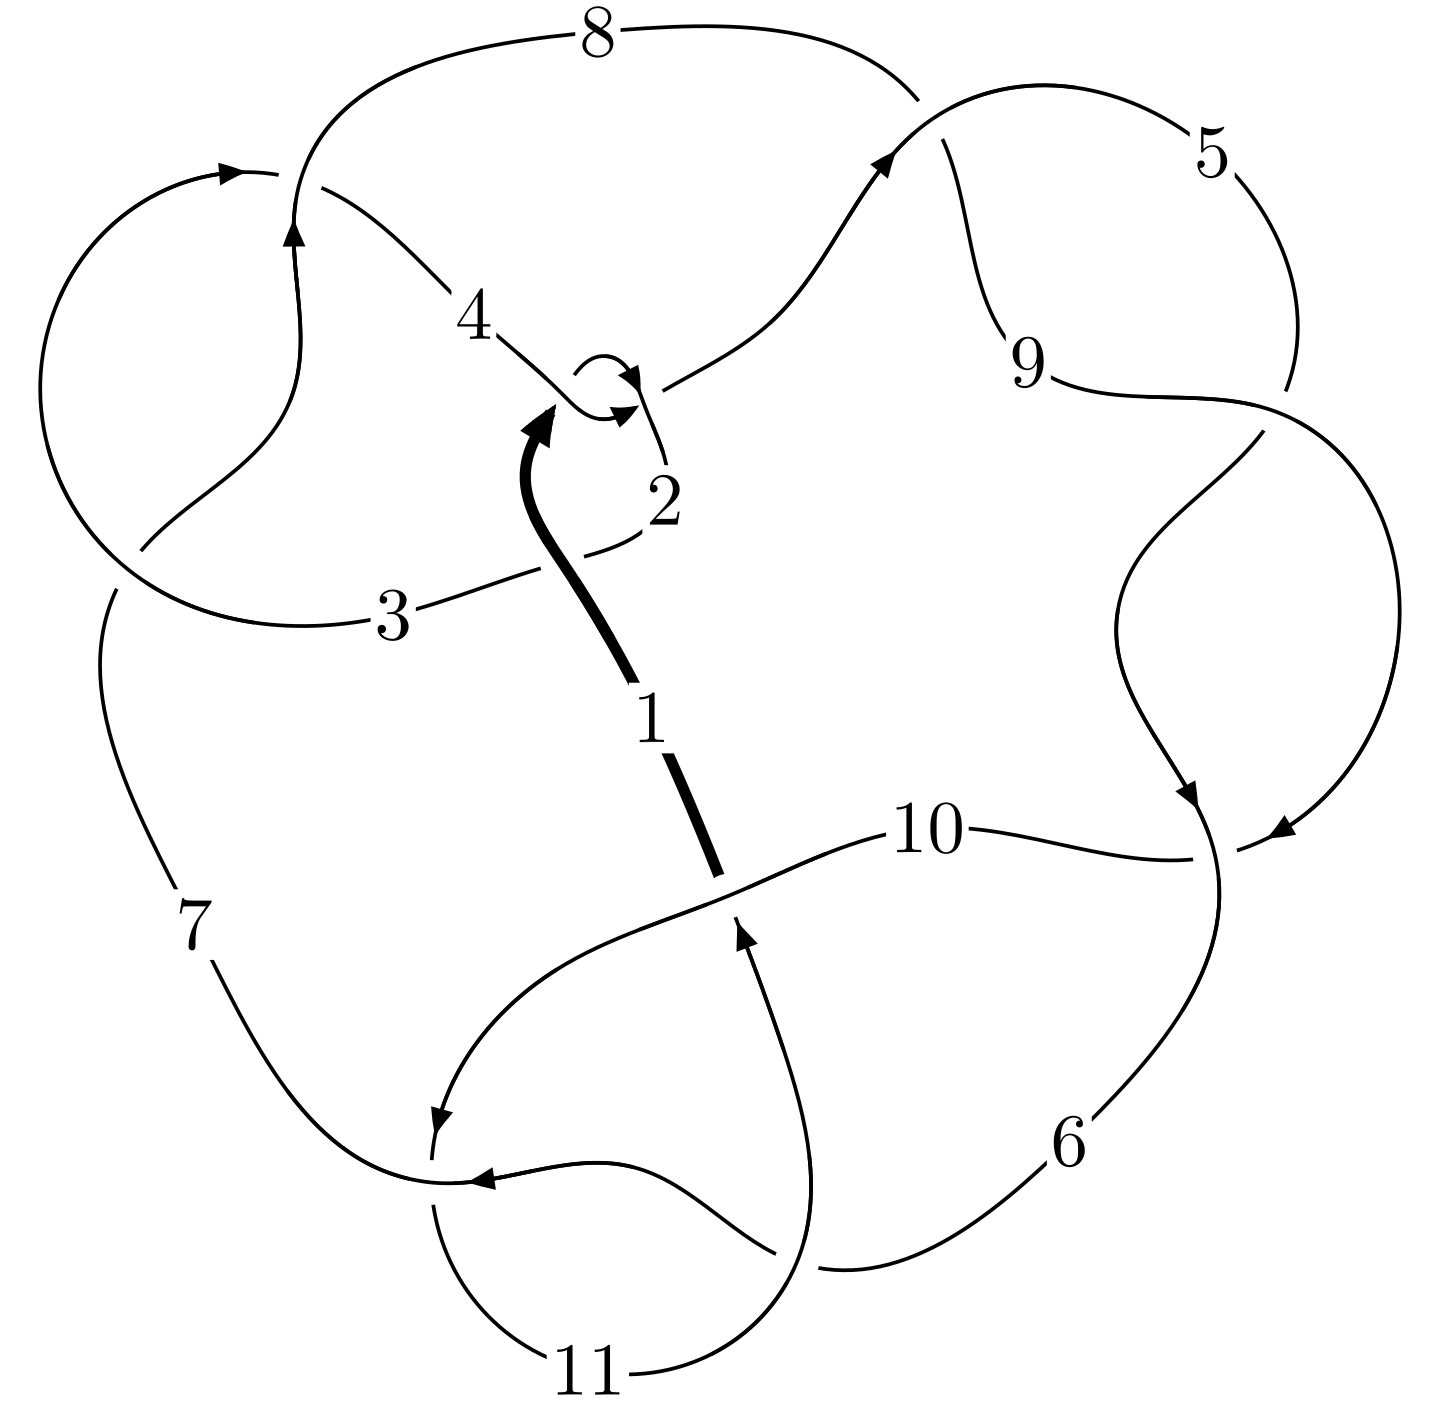
\includegraphics[width=112pt]{../../../GIT/diagram.site/Diagrams/png/282_11a_33.png}\\
\ \ \ A knot diagram\footnotemark}&
\allowdisplaybreaks
\textbf{Linearized knot diagam} \\
\cline{2-2}
 &
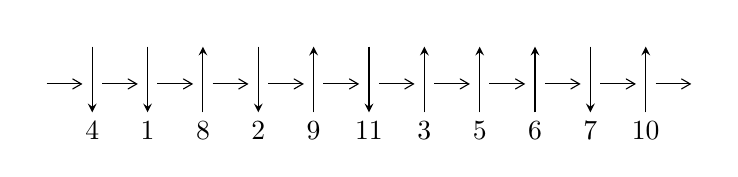
\begin{tikzpicture}[x=20pt, y=17pt]
	% nodes
	\node (C0) at (0, 0) {};
	\node (C1) at (1, 0) {};
	\node (C1U) at (1, +1) {};
	\node (C1D) at (1, -1) {4};

	\node (C2) at (2, 0) {};
	\node (C2U) at (2, +1) {};
	\node (C2D) at (2, -1) {1};

	\node (C3) at (3, 0) {};
	\node (C3U) at (3, +1) {};
	\node (C3D) at (3, -1) {8};

	\node (C4) at (4, 0) {};
	\node (C4U) at (4, +1) {};
	\node (C4D) at (4, -1) {2};

	\node (C5) at (5, 0) {};
	\node (C5U) at (5, +1) {};
	\node (C5D) at (5, -1) {9};

	\node (C6) at (6, 0) {};
	\node (C6U) at (6, +1) {};
	\node (C6D) at (6, -1) {11};

	\node (C7) at (7, 0) {};
	\node (C7U) at (7, +1) {};
	\node (C7D) at (7, -1) {3};

	\node (C8) at (8, 0) {};
	\node (C8U) at (8, +1) {};
	\node (C8D) at (8, -1) {5};

	\node (C9) at (9, 0) {};
	\node (C9U) at (9, +1) {};
	\node (C9D) at (9, -1) {6};

	\node (C10) at (10, 0) {};
	\node (C10U) at (10, +1) {};
	\node (C10D) at (10, -1) {7};

	\node (C11) at (11, 0) {};
	\node (C11U) at (11, +1) {};
	\node (C11D) at (11, -1) {10};
	\node (C12) at (12, 0) {};

	% arrows
	\draw[->,>={angle 60}]
	(C0) edge (C1) (C1) edge (C2) (C2) edge (C3) (C3) edge (C4) (C4) edge (C5) (C5) edge (C6) (C6) edge (C7) (C7) edge (C8) (C8) edge (C9) (C9) edge (C10) (C10) edge (C11) (C11) edge (C12) ;	\draw[->,>=stealth]
	(C1U) edge (C1D) (C2U) edge (C2D) (C3D) edge (C3U) (C4U) edge (C4D) (C5D) edge (C5U) (C6U) edge (C6D) (C7D) edge (C7U) (C8D) edge (C8U) (C9D) edge (C9U) (C10U) edge (C10D) (C11D) edge (C11U) ;
	\end{tikzpicture} \\
\hhline{~~} \\& 
\textbf{Solving Sequence} \\ \cline{2-2} 
 &
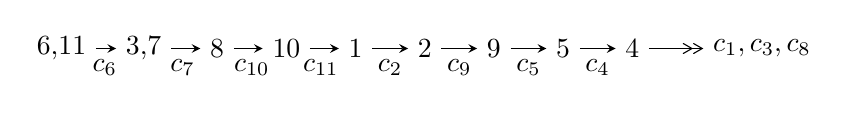
\begin{tikzpicture}[x=25pt, y=7pt]
	% node
	\node (A0) at (-1/8, 0) {6,11};
	\node (A1) at (17/16, 0) {3,7};
	\node (A2) at (17/8, 0) {8};
	\node (A3) at (25/8, 0) {10};
	\node (A4) at (33/8, 0) {1};
	\node (A5) at (41/8, 0) {2};
	\node (A6) at (49/8, 0) {9};
	\node (A7) at (57/8, 0) {5};
	\node (A8) at (65/8, 0) {4};
	\node (C1) at (1/2, -1) {$c_{6}$};
	\node (C2) at (13/8, -1) {$c_{7}$};
	\node (C3) at (21/8, -1) {$c_{10}$};
	\node (C4) at (29/8, -1) {$c_{11}$};
	\node (C5) at (37/8, -1) {$c_{2}$};
	\node (C6) at (45/8, -1) {$c_{9}$};
	\node (C7) at (53/8, -1) {$c_{5}$};
	\node (C8) at (61/8, -1) {$c_{4}$};
	\node (A9) at (10, 0) {$c_{1},c_{3},c_{8}$};

	% edge
	\draw[->,>=stealth]	
	(A0) edge (A1) (A1) edge (A2) (A2) edge (A3) (A3) edge (A4) (A4) edge (A5) (A5) edge (A6) (A6) edge (A7) (A7) edge (A8) ;
	\draw[->>,>={angle 60}]	
	(A8) edge (A9);
\end{tikzpicture} \\ 

\end{tabular} \\

\footnotetext{
The image of knot diagram is generated by the software ``\textbf{Draw programme}" developed by Andrew Bartholomew(\url{http://www.layer8.co.uk/maths/draw/index.htm\#Running-draw}), where we modified some parts for our purpose(\url{https://github.com/CATsTAILs/LinksPainter}).
}\phantom \\ \newline 
\centering \textbf{Ideals for irreducible components\footnotemark of $X_{\text{par}}$} 
 
\begin{align*}
I^u_{1}&=\langle 
- u^{50}- u^{49}+\cdots+b- u,\;u^{50}- u^{49}+\cdots+a-1,\;u^{52}-2 u^{51}+\cdots+u-1\rangle \\
I^u_{2}&=\langle 
- u^4- u^3- u^2+b,\;- u^2+a- u-1,\;u^5+u^4+2 u^3+u^2+u+1\rangle \\
\\
\end{align*}
\raggedright * 2 irreducible components of $\dim_{\mathbb{C}}=0$, with total 57 representations.\\
\footnotetext{All coefficients of polynomials are rational numbers. But the coefficients are sometimes approximated in decimal forms when there is not enough margin.}
\newpage
\renewcommand{\arraystretch}{1}
\centering \section*{I. $I^u_{1}= \langle - u^{50}- u^{49}+\cdots+b- u,\;u^{50}- u^{49}+\cdots+a-1,\;u^{52}-2 u^{51}+\cdots+u-1 \rangle$}
\flushleft \textbf{(i) Arc colorings}\\
\begin{tabular}{m{7pt} m{180pt} m{7pt} m{180pt} }
\flushright $a_{6}=$&$\begin{pmatrix}1\\0\end{pmatrix}$ \\
\flushright $a_{11}=$&$\begin{pmatrix}0\\u\end{pmatrix}$ \\
\flushright $a_{3}=$&$\begin{pmatrix}- u^{50}+u^{49}+\cdots-2 u+1\\u^{50}+u^{49}+\cdots+2 u^2+u\end{pmatrix}$ \\
\flushright $a_{7}=$&$\begin{pmatrix}1\\u^2\end{pmatrix}$ \\
\flushright $a_{8}=$&$\begin{pmatrix}u^9+2 u^7+u^5-2 u^3- u\\- u^9-3 u^7-3 u^5+u\end{pmatrix}$ \\
\flushright $a_{10}=$&$\begin{pmatrix}u\\u^3+u\end{pmatrix}$ \\
\flushright $a_{1}=$&$\begin{pmatrix}u^3\\u^5+u^3+u\end{pmatrix}$ \\
\flushright $a_{2}=$&$\begin{pmatrix}u^{47}- u^{46}+\cdots- u^2-2 u\\u^{49}- u^{48}+\cdots+6 u^4+2 u^2\end{pmatrix}$ \\
\flushright $a_{9}=$&$\begin{pmatrix}- u^3\\u^3+u\end{pmatrix}$ \\
\flushright $a_{5}=$&$\begin{pmatrix}- u^6- u^4+1\\u^6+2 u^4+u^2\end{pmatrix}$ \\
\flushright $a_{4}=$&$\begin{pmatrix}u^{50}- u^{49}+\cdots-2 u^2-2 u\\- u^{50}+u^{49}+\cdots- u^3+2 u^2\end{pmatrix}$\\ \flushright $a_{4}=$&$\begin{pmatrix}u^{50}- u^{49}+\cdots-2 u^2-2 u\\- u^{50}+u^{49}+\cdots- u^3+2 u^2\end{pmatrix}$\\&\end{tabular}
\flushleft \textbf{(ii) Obstruction class $= -1$}\\~\\
\flushleft \textbf{(iii) Cusp Shapes $= -4 u^{51}+5 u^{50}+\cdots+2 u-1$}\\~\\
\newpage\renewcommand{\arraystretch}{1}
\flushleft \textbf{(iv) u-Polynomials at the component}\newline \\
\begin{tabular}{m{50pt}|m{274pt}}
Crossings & \hspace{64pt}u-Polynomials at each crossing \\
\hline $$\begin{aligned}c_{1},c_{4}\end{aligned}$$&$\begin{aligned}
&u^{52}-6 u^{51}+\cdots+5 u-1
\end{aligned}$\\
\hline $$\begin{aligned}c_{2}\end{aligned}$$&$\begin{aligned}
&u^{52}+22 u^{51}+\cdots-11 u+1
\end{aligned}$\\
\hline $$\begin{aligned}c_{3},c_{7}\end{aligned}$$&$\begin{aligned}
&u^{52}+u^{51}+\cdots-232 u^2+32
\end{aligned}$\\
\hline $$\begin{aligned}c_{5},c_{8},c_{9}\end{aligned}$$&$\begin{aligned}
&u^{52}-2 u^{51}+\cdots-25 u-17
\end{aligned}$\\
\hline $$\begin{aligned}c_{6},c_{10}\end{aligned}$$&$\begin{aligned}
&u^{52}+2 u^{51}+\cdots- u-1
\end{aligned}$\\
\hline $$\begin{aligned}c_{11}\end{aligned}$$&$\begin{aligned}
&u^{52}-30 u^{51}+\cdots-5 u+1
\end{aligned}$\\
\hline
\end{tabular}\\~\\
\newpage\renewcommand{\arraystretch}{1}
\flushleft \textbf{(v) Riley Polynomials at the component}\newline \\
\begin{tabular}{m{50pt}|m{274pt}}
Crossings & \hspace{64pt}Riley Polynomials at each crossing \\
\hline $$\begin{aligned}c_{1},c_{4}\end{aligned}$$&$\begin{aligned}
&y^{52}-22 y^{51}+\cdots+11 y+1
\end{aligned}$\\
\hline $$\begin{aligned}c_{2}\end{aligned}$$&$\begin{aligned}
&y^{52}+22 y^{51}+\cdots-349 y+1
\end{aligned}$\\
\hline $$\begin{aligned}c_{3},c_{7}\end{aligned}$$&$\begin{aligned}
&y^{52}-33 y^{51}+\cdots-14848 y+1024
\end{aligned}$\\
\hline $$\begin{aligned}c_{5},c_{8},c_{9}\end{aligned}$$&$\begin{aligned}
&y^{52}-58 y^{51}+\cdots-2291 y+289
\end{aligned}$\\
\hline $$\begin{aligned}c_{6},c_{10}\end{aligned}$$&$\begin{aligned}
&y^{52}+30 y^{51}+\cdots+5 y+1
\end{aligned}$\\
\hline $$\begin{aligned}c_{11}\end{aligned}$$&$\begin{aligned}
&y^{52}-14 y^{51}+\cdots+21 y+1
\end{aligned}$\\
\hline
\end{tabular}\\~\\
\newpage\flushleft \textbf{(vi) Complex Volumes and Cusp Shapes}
$$\begin{array}{c|c|c}  
\text{Solutions to }I^u_{1}& \I (\text{vol} + \sqrt{-1}CS) & \text{Cusp shape}\\
 \hline 
\begin{aligned}
u &= \phantom{-}0.280725 + 0.984494 I \\
a &= \phantom{-}0.654643 + 0.042402 I \\
b &= -0.595405 - 0.490264 I\end{aligned}
 & \phantom{-}0.986067 - 0.922209 I & \phantom{-}5.57805 + 0.78370 I \\ \hline\begin{aligned}
u &= \phantom{-}0.280725 - 0.984494 I \\
a &= \phantom{-}0.654643 - 0.042402 I \\
b &= -0.595405 + 0.490264 I\end{aligned}
 & \phantom{-}0.986067 + 0.922209 I & \phantom{-}5.57805 - 0.78370 I \\ \hline\begin{aligned}
u &= -0.377650 + 0.954360 I \\
a &= \phantom{-}2.41555 - 1.60256 I \\
b &= -2.28692 - 0.23404 I\end{aligned}
 & -0.88919 + 2.40502 I & \phantom{-}4.23135 - 7.49678 I \\ \hline\begin{aligned}
u &= -0.377650 - 0.954360 I \\
a &= \phantom{-}2.41555 + 1.60256 I \\
b &= -2.28692 + 0.23404 I\end{aligned}
 & -0.88919 - 2.40502 I & \phantom{-}4.23135 + 7.49678 I \\ \hline\begin{aligned}
u &= \phantom{-}0.508227 + 0.805847 I \\
a &= -0.742914 + 0.724717 I \\
b &= \phantom{-}0.658582 - 0.670829 I\end{aligned}
 & -0.0437779 - 0.0269953 I & \phantom{-}1.92084 + 0.19212 I \\ \hline\begin{aligned}
u &= \phantom{-}0.508227 - 0.805847 I \\
a &= -0.742914 - 0.724717 I \\
b &= \phantom{-}0.658582 + 0.670829 I\end{aligned}
 & -0.0437779 + 0.0269953 I & \phantom{-}1.92084 - 0.19212 I \\ \hline\begin{aligned}
u &= \phantom{-}0.422777 + 0.995937 I \\
a &= -0.819376 - 0.080332 I \\
b &= \phantom{-}1.105830 + 0.262915 I\end{aligned}
 & -0.04250 - 4.54357 I & \phantom{-}1.88793 + 7.26372 I \\ \hline\begin{aligned}
u &= \phantom{-}0.422777 - 0.995937 I \\
a &= -0.819376 + 0.080332 I \\
b &= \phantom{-}1.105830 - 0.262915 I\end{aligned}
 & -0.04250 + 4.54357 I & \phantom{-}1.88793 - 7.26372 I \\ \hline\begin{aligned}
u &= \phantom{-}0.889760 + 0.039446 I \\
a &= -0.980477 + 0.475985 I \\
b &= -2.22766 - 0.07116 I\end{aligned}
 & \phantom{-}9.80914 + 2.73925 I & \phantom{-}5.98913 - 0.86649 I \\ \hline\begin{aligned}
u &= \phantom{-}0.889760 - 0.039446 I \\
a &= -0.980477 - 0.475985 I \\
b &= -2.22766 + 0.07116 I\end{aligned}
 & \phantom{-}9.80914 - 2.73925 I & \phantom{-}5.98913 + 0.86649 I\\
 \hline 
 \end{array}$$\newpage$$\begin{array}{c|c|c}  
\text{Solutions to }I^u_{1}& \I (\text{vol} + \sqrt{-1}CS) & \text{Cusp shape}\\
 \hline 
\begin{aligned}
u &= \phantom{-}0.885810 + 0.066307 I \\
a &= \phantom{-}0.908664 - 0.767749 I \\
b &= \phantom{-}2.15596 + 0.13200 I\end{aligned}
 & \phantom{-}7.94022 + 8.91057 I & \phantom{-}3.69132 - 5.27448 I \\ \hline\begin{aligned}
u &= \phantom{-}0.885810 - 0.066307 I \\
a &= \phantom{-}0.908664 + 0.767749 I \\
b &= \phantom{-}2.15596 - 0.13200 I\end{aligned}
 & \phantom{-}7.94022 - 8.91057 I & \phantom{-}3.69132 + 5.27448 I \\ \hline\begin{aligned}
u &= -0.165811 + 1.121200 I \\
a &= \phantom{-}1.83757 - 0.40541 I \\
b &= -1.130520 - 0.544612 I\end{aligned}
 & \phantom{-}5.10574 - 3.32861 I & \phantom{-}8.68775 + 2.82645 I \\ \hline\begin{aligned}
u &= -0.165811 - 1.121200 I \\
a &= \phantom{-}1.83757 + 0.40541 I \\
b &= -1.130520 + 0.544612 I\end{aligned}
 & \phantom{-}5.10574 + 3.32861 I & \phantom{-}8.68775 - 2.82645 I \\ \hline\begin{aligned}
u &= -0.860610 + 0.023085 I \\
a &= -0.066448 - 0.251952 I \\
b &= \phantom{-}0.153988 + 0.972076 I\end{aligned}
 & \phantom{-}4.28726 - 2.50747 I & \phantom{-}2.75724 + 2.68671 I \\ \hline\begin{aligned}
u &= -0.860610 - 0.023085 I \\
a &= -0.066448 + 0.251952 I \\
b &= \phantom{-}0.153988 - 0.972076 I\end{aligned}
 & \phantom{-}4.28726 + 2.50747 I & \phantom{-}2.75724 - 2.68671 I \\ \hline\begin{aligned}
u &= \phantom{-}0.529646 + 0.675176 I \\
a &= \phantom{-}0.520778 - 1.165510 I \\
b &= -0.287257 + 0.910625 I\end{aligned}
 & -0.40755 - 4.20725 I & \phantom{-}0.31053 + 6.85372 I \\ \hline\begin{aligned}
u &= \phantom{-}0.529646 - 0.675176 I \\
a &= \phantom{-}0.520778 + 1.165510 I \\
b &= -0.287257 - 0.910625 I\end{aligned}
 & -0.40755 + 4.20725 I & \phantom{-}0.31053 - 6.85372 I \\ \hline\begin{aligned}
u &= -0.511753 + 1.024350 I \\
a &= \phantom{-}1.26087 - 1.89055 I \\
b &= -1.78707 + 0.70393 I\end{aligned}
 & \phantom{-}2.58119 + 9.82991 I & \phantom{-}3.68059 - 9.74649 I \\ \hline\begin{aligned}
u &= -0.511753 - 1.024350 I \\
a &= \phantom{-}1.26087 + 1.89055 I \\
b &= -1.78707 - 0.70393 I\end{aligned}
 & \phantom{-}2.58119 - 9.82991 I & \phantom{-}3.68059 + 9.74649 I\\
 \hline 
 \end{array}$$\newpage$$\begin{array}{c|c|c}  
\text{Solutions to }I^u_{1}& \I (\text{vol} + \sqrt{-1}CS) & \text{Cusp shape}\\
 \hline 
\begin{aligned}
u &= \phantom{-}0.848851\phantom{ +0.000000I} \\
a &= \phantom{-}1.68388\phantom{ +0.000000I} \\
b &= \phantom{-}2.26297\phantom{ +0.000000I}\end{aligned}
 & \phantom{-}2.68190\phantom{ +0.000000I} & \phantom{-}3.52270\phantom{ +0.000000I} \\ \hline\begin{aligned}
u &= -0.245968 + 1.124790 I \\
a &= -1.86661 + 0.47174 I \\
b &= \phantom{-}1.248780 + 0.497288 I\end{aligned}
 & \phantom{-}5.88940 + 2.23703 I & \phantom{-}9.81871 - 3.17171 I \\ \hline\begin{aligned}
u &= -0.245968 - 1.124790 I \\
a &= -1.86661 - 0.47174 I \\
b &= \phantom{-}1.248780 - 0.497288 I\end{aligned}
 & \phantom{-}5.88940 - 2.23703 I & \phantom{-}9.81871 + 3.17171 I \\ \hline\begin{aligned}
u &= -0.460826 + 1.063150 I \\
a &= -1.28681 + 1.46544 I \\
b &= \phantom{-}1.53108 - 0.39330 I\end{aligned}
 & \phantom{-}4.31532 + 4.63289 I & \phantom{-}7.37710 - 5.03996 I \\ \hline\begin{aligned}
u &= -0.460826 - 1.063150 I \\
a &= -1.28681 - 1.46544 I \\
b &= \phantom{-}1.53108 + 0.39330 I\end{aligned}
 & \phantom{-}4.31532 - 4.63289 I & \phantom{-}7.37710 + 5.03996 I \\ \hline\begin{aligned}
u &= \phantom{-}0.249339 + 0.786720 I \\
a &= \phantom{-}0.457886 + 0.514045 I \\
b &= -0.154878 - 0.504949 I\end{aligned}
 & \phantom{-}0.450033 - 1.234720 I & \phantom{-}4.74084 + 5.50358 I \\ \hline\begin{aligned}
u &= \phantom{-}0.249339 - 0.786720 I \\
a &= \phantom{-}0.457886 - 0.514045 I \\
b &= -0.154878 + 0.504949 I\end{aligned}
 & \phantom{-}0.450033 + 1.234720 I & \phantom{-}4.74084 - 5.50358 I \\ \hline\begin{aligned}
u &= -0.457667 + 1.181360 I \\
a &= -0.427283 + 0.598681 I \\
b &= \phantom{-}0.526120 - 0.236335 I\end{aligned}
 & \phantom{-}5.00504 + 4.26604 I & \phantom{-0.000000 } 0 \\ \hline\begin{aligned}
u &= -0.457667 - 1.181360 I \\
a &= -0.427283 - 0.598681 I \\
b &= \phantom{-}0.526120 + 0.236335 I\end{aligned}
 & \phantom{-}5.00504 - 4.26604 I & \phantom{-0.000000 } 0 \\ \hline\begin{aligned}
u &= -0.626363 + 0.365158 I \\
a &= \phantom{-}0.331365 - 0.906721 I \\
b &= -1.48252 + 0.06887 I\end{aligned}
 & \phantom{-}0.72885 - 5.40223 I & \phantom{-}0.76570 + 5.29849 I\\
 \hline 
 \end{array}$$\newpage$$\begin{array}{c|c|c}  
\text{Solutions to }I^u_{1}& \I (\text{vol} + \sqrt{-1}CS) & \text{Cusp shape}\\
 \hline 
\begin{aligned}
u &= -0.626363 - 0.365158 I \\
a &= \phantom{-}0.331365 + 0.906721 I \\
b &= -1.48252 - 0.06887 I\end{aligned}
 & \phantom{-}0.72885 + 5.40223 I & \phantom{-}0.76570 - 5.29849 I \\ \hline\begin{aligned}
u &= -0.707531\phantom{ +0.000000I} \\
a &= -0.0272312\phantom{ +0.000000I} \\
b &= \phantom{-}0.597785\phantom{ +0.000000I}\end{aligned}
 & \phantom{-}1.69898\phantom{ +0.000000I} & \phantom{-}7.12320\phantom{ +0.000000I} \\ \hline\begin{aligned}
u &= \phantom{-}0.463049 + 1.238040 I \\
a &= -2.55511 - 0.88903 I \\
b &= \phantom{-}3.29992 - 1.71101 I\end{aligned}
 & \phantom{-}6.39075 - 4.67632 I & \phantom{-0.000000 } 0 \\ \hline\begin{aligned}
u &= \phantom{-}0.463049 - 1.238040 I \\
a &= -2.55511 + 0.88903 I \\
b &= \phantom{-}3.29992 + 1.71101 I\end{aligned}
 & \phantom{-}6.39075 + 4.67632 I & \phantom{-0.000000 } 0 \\ \hline\begin{aligned}
u &= -0.451975 + 1.246010 I \\
a &= -0.987426 - 0.642867 I \\
b &= \phantom{-}0.437332 + 0.795179 I\end{aligned}
 & \phantom{-}8.11586 + 2.13977 I & \phantom{-0.000000 } 0 \\ \hline\begin{aligned}
u &= -0.451975 - 1.246010 I \\
a &= -0.987426 + 0.642867 I \\
b &= \phantom{-}0.437332 - 0.795179 I\end{aligned}
 & \phantom{-}8.11586 - 2.13977 I & \phantom{-0.000000 } 0 \\ \hline\begin{aligned}
u &= -0.475337 + 1.240760 I \\
a &= \phantom{-}0.772991 + 0.898748 I \\
b &= -0.203290 - 0.904404 I\end{aligned}
 & \phantom{-}7.94604 + 7.28946 I & \phantom{-0.000000 } 0 \\ \hline\begin{aligned}
u &= -0.475337 - 1.240760 I \\
a &= \phantom{-}0.772991 - 0.898748 I \\
b &= -0.203290 + 0.904404 I\end{aligned}
 & \phantom{-}7.94604 - 7.28946 I & \phantom{-0.000000 } 0 \\ \hline\begin{aligned}
u &= -0.625397 + 0.228924 I \\
a &= -0.107645 + 0.510658 I \\
b &= \phantom{-}1.145420 + 0.098339 I\end{aligned}
 & \phantom{-}1.98030 - 0.48005 I & \phantom{-}3.97181 + 0.10468 I \\ \hline\begin{aligned}
u &= -0.625397 - 0.228924 I \\
a &= -0.107645 - 0.510658 I \\
b &= \phantom{-}1.145420 - 0.098339 I\end{aligned}
 & \phantom{-}1.98030 + 0.48005 I & \phantom{-}3.97181 - 0.10468 I\\
 \hline 
 \end{array}$$\newpage$$\begin{array}{c|c|c}  
\text{Solutions to }I^u_{1}& \I (\text{vol} + \sqrt{-1}CS) & \text{Cusp shape}\\
 \hline 
\begin{aligned}
u &= \phantom{-}0.427798 + 1.265370 I \\
a &= -1.75085 - 0.81280 I \\
b &= \phantom{-}1.97471 - 1.35185 I\end{aligned}
 & \phantom{-}12.02740 + 4.30908 I & \phantom{-0.000000 } 0 \\ \hline\begin{aligned}
u &= \phantom{-}0.427798 - 1.265370 I \\
a &= -1.75085 + 0.81280 I \\
b &= \phantom{-}1.97471 + 1.35185 I\end{aligned}
 & \phantom{-}12.02740 - 4.30908 I & \phantom{-0.000000 } 0 \\ \hline\begin{aligned}
u &= \phantom{-}0.500173 + 1.244000 I \\
a &= -2.42580 - 1.28995 I \\
b &= \phantom{-}3.39254 - 0.69209 I\end{aligned}
 & \phantom{-}11.4963 - 13.8946 I & \phantom{-0.000000 } 0 \\ \hline\begin{aligned}
u &= \phantom{-}0.500173 - 1.244000 I \\
a &= -2.42580 + 1.28995 I \\
b &= \phantom{-}3.39254 + 0.69209 I\end{aligned}
 & \phantom{-}11.4963 + 13.8946 I & \phantom{-0.000000 } 0 \\ \hline\begin{aligned}
u &= \phantom{-}0.445030 + 1.264870 I \\
a &= \phantom{-}1.99511 + 0.91581 I \\
b &= -2.37247 + 1.31494 I\end{aligned}
 & \phantom{-}13.79830 - 1.96896 I & \phantom{-0.000000 } 0 \\ \hline\begin{aligned}
u &= \phantom{-}0.445030 - 1.264870 I \\
a &= \phantom{-}1.99511 - 0.91581 I \\
b &= -2.37247 - 1.31494 I\end{aligned}
 & \phantom{-}13.79830 + 1.96896 I & \phantom{-0.000000 } 0 \\ \hline\begin{aligned}
u &= \phantom{-}0.488189 + 1.251510 I \\
a &= \phantom{-}2.39866 + 1.22603 I \\
b &= -3.25277 + 0.88645 I\end{aligned}
 & \phantom{-}13.4799 - 7.6731 I & \phantom{-0.000000 } 0 \\ \hline\begin{aligned}
u &= \phantom{-}0.488189 - 1.251510 I \\
a &= \phantom{-}2.39866 - 1.22603 I \\
b &= -3.25277 - 0.88645 I\end{aligned}
 & \phantom{-}13.4799 + 7.6731 I & \phantom{-0.000000 } 0 \\ \hline\begin{aligned}
u &= -0.287199 + 0.547902 I \\
a &= -0.76127 - 1.80488 I \\
b &= -0.88257 + 1.12082 I\end{aligned}
 & -2.08809 + 0.78607 I & -3.98062 + 1.52380 I \\ \hline\begin{aligned}
u &= -0.287199 - 0.547902 I \\
a &= -0.76127 + 1.80488 I \\
b &= -0.88257 - 1.12082 I\end{aligned}
 & -2.08809 - 0.78607 I & -3.98062 - 1.52380 I\\
 \hline 
 \end{array}$$\newpage$$\begin{array}{c|c|c}  
\text{Solutions to }I^u_{1}& \I (\text{vol} + \sqrt{-1}CS) & \text{Cusp shape}\\
 \hline 
\begin{aligned}
u &= \phantom{-}0.385374 + 0.321628 I \\
a &= -0.10441 - 1.83686 I \\
b &= \phantom{-}0.102691 + 0.571781 I\end{aligned}
 & -1.79468 + 0.95889 I & -4.14280 - 1.57937 I \\ \hline\begin{aligned}
u &= \phantom{-}0.385374 - 0.321628 I \\
a &= -0.10441 + 1.83686 I \\
b &= \phantom{-}0.102691 - 0.571781 I\end{aligned}
 & -1.79468 - 0.95889 I & -4.14280 + 1.57937 I\\
 \hline 
 \end{array}$$\newpage\newpage\renewcommand{\arraystretch}{1}
\centering \section*{II. $I^u_{2}= \langle - u^4- u^3- u^2+b,\;- u^2+a- u-1,\;u^5+u^4+2 u^3+u^2+u+1 \rangle$}
\flushleft \textbf{(i) Arc colorings}\\
\begin{tabular}{m{7pt} m{180pt} m{7pt} m{180pt} }
\flushright $a_{6}=$&$\begin{pmatrix}1\\0\end{pmatrix}$ \\
\flushright $a_{11}=$&$\begin{pmatrix}0\\u\end{pmatrix}$ \\
\flushright $a_{3}=$&$\begin{pmatrix}u^2+u+1\\u^4+u^3+u^2\end{pmatrix}$ \\
\flushright $a_{7}=$&$\begin{pmatrix}1\\u^2\end{pmatrix}$ \\
\flushright $a_{8}=$&$\begin{pmatrix}1\\u^2\end{pmatrix}$ \\
\flushright $a_{10}=$&$\begin{pmatrix}u\\u^3+u\end{pmatrix}$ \\
\flushright $a_{1}=$&$\begin{pmatrix}u^3\\- u^4- u^3- u^2-1\end{pmatrix}$ \\
\flushright $a_{2}=$&$\begin{pmatrix}u^3+u^2+u+1\\-1\end{pmatrix}$ \\
\flushright $a_{9}=$&$\begin{pmatrix}- u^3\\u^3+u\end{pmatrix}$ \\
\flushright $a_{5}=$&$\begin{pmatrix}- u^3\\u^4+u^3+u^2+1\end{pmatrix}$ \\
\flushright $a_{4}=$&$\begin{pmatrix}u^2+u+1\\u^4+u^3+u^2\end{pmatrix}$\\ \flushright $a_{4}=$&$\begin{pmatrix}u^2+u+1\\u^4+u^3+u^2\end{pmatrix}$\\&\end{tabular}
\flushleft \textbf{(ii) Obstruction class $= 1$}\\~\\
\flushleft \textbf{(iii) Cusp Shapes $= -2 u^4+u^3+2 u$}\\~\\
\newpage\renewcommand{\arraystretch}{1}
\flushleft \textbf{(iv) u-Polynomials at the component}\newline \\
\begin{tabular}{m{50pt}|m{274pt}}
Crossings & \hspace{64pt}u-Polynomials at each crossing \\
\hline $$\begin{aligned}c_{1}\end{aligned}$$&$\begin{aligned}
&(u-1)^5
\end{aligned}$\\
\hline $$\begin{aligned}c_{2},c_{4}\end{aligned}$$&$\begin{aligned}
&(u+1)^5
\end{aligned}$\\
\hline $$\begin{aligned}c_{3},c_{7}\end{aligned}$$&$\begin{aligned}
&u^5
\end{aligned}$\\
\hline $$\begin{aligned}c_{5}\end{aligned}$$&$\begin{aligned}
&u^5- u^4-2 u^3+u^2+u+1
\end{aligned}$\\
\hline $$\begin{aligned}c_{6}\end{aligned}$$&$\begin{aligned}
&u^5+u^4+2 u^3+u^2+u+1
\end{aligned}$\\
\hline $$\begin{aligned}c_{8},c_{9}\end{aligned}$$&$\begin{aligned}
&u^5+u^4-2 u^3- u^2+u-1
\end{aligned}$\\
\hline $$\begin{aligned}c_{10}\end{aligned}$$&$\begin{aligned}
&u^5- u^4+2 u^3- u^2+u-1
\end{aligned}$\\
\hline $$\begin{aligned}c_{11}\end{aligned}$$&$\begin{aligned}
&u^5-3 u^4+4 u^3- u^2- u+1
\end{aligned}$\\
\hline
\end{tabular}\\~\\
\newpage\renewcommand{\arraystretch}{1}
\flushleft \textbf{(v) Riley Polynomials at the component}\newline \\
\begin{tabular}{m{50pt}|m{274pt}}
Crossings & \hspace{64pt}Riley Polynomials at each crossing \\
\hline $$\begin{aligned}c_{1},c_{2},c_{4}\end{aligned}$$&$\begin{aligned}
&(y-1)^5
\end{aligned}$\\
\hline $$\begin{aligned}c_{3},c_{7}\end{aligned}$$&$\begin{aligned}
&y^5
\end{aligned}$\\
\hline $$\begin{aligned}c_{5},c_{8},c_{9}\end{aligned}$$&$\begin{aligned}
&y^5-5 y^4+8 y^3-3 y^2- y-1
\end{aligned}$\\
\hline $$\begin{aligned}c_{6},c_{10}\end{aligned}$$&$\begin{aligned}
&y^5+3 y^4+4 y^3+y^2- y-1
\end{aligned}$\\
\hline $$\begin{aligned}c_{11}\end{aligned}$$&$\begin{aligned}
&y^5- y^4+8 y^3-3 y^2+3 y-1
\end{aligned}$\\
\hline
\end{tabular}\\~\\
\newpage\flushleft \textbf{(vi) Complex Volumes and Cusp Shapes}
$$\begin{array}{c|c|c}  
\text{Solutions to }I^u_{2}& \I (\text{vol} + \sqrt{-1}CS) & \text{Cusp shape}\\
 \hline 
\begin{aligned}
u &= \phantom{-}0.339110 + 0.822375 I \\
a &= \phantom{-}0.77780 + 1.38013 I \\
b &= -1.206350 - 0.340852 I\end{aligned}
 & -1.31583 - 1.53058 I & \phantom{-}0.02124 + 2.62456 I \\ \hline\begin{aligned}
u &= \phantom{-}0.339110 - 0.822375 I \\
a &= \phantom{-}0.77780 - 1.38013 I \\
b &= -1.206350 + 0.340852 I\end{aligned}
 & -1.31583 + 1.53058 I & \phantom{-}0.02124 - 2.62456 I \\ \hline\begin{aligned}
u &= -0.766826\phantom{ +0.000000I} \\
a &= \phantom{-}0.821196\phantom{ +0.000000I} \\
b &= \phantom{-}0.482881\phantom{ +0.000000I}\end{aligned}
 & \phantom{-}0.756147\phantom{ +0.000000I} & -2.67610\phantom{ +0.000000I} \\ \hline\begin{aligned}
u &= -0.455697 + 1.200150 I \\
a &= -0.688402 + 0.106340 I \\
b &= \phantom{-}0.964913 + 0.621896 I\end{aligned}
 & \phantom{-}4.22763 + 4.40083 I & \phantom{-}0.31681 - 3.97407 I \\ \hline\begin{aligned}
u &= -0.455697 - 1.200150 I \\
a &= -0.688402 - 0.106340 I \\
b &= \phantom{-}0.964913 - 0.621896 I\end{aligned}
 & \phantom{-}4.22763 - 4.40083 I & \phantom{-}0.31681 + 3.97407 I\\
 \hline 
 \end{array}$$\newpage
\newpage\renewcommand{\arraystretch}{1}
\centering \section*{ III. u-Polynomials}
\begin{tabular}{m{50pt}|m{274pt}}
Crossings & \hspace{64pt}u-Polynomials at each crossing \\
\hline $$\begin{aligned}c_{1}\end{aligned}$$&$\begin{aligned}
&((u-1)^5)(u^{52}-6 u^{51}+\cdots+5 u-1)
\end{aligned}$\\
\hline $$\begin{aligned}c_{2}\end{aligned}$$&$\begin{aligned}
&((u+1)^5)(u^{52}+22 u^{51}+\cdots-11 u+1)
\end{aligned}$\\
\hline $$\begin{aligned}c_{3},c_{7}\end{aligned}$$&$\begin{aligned}
&u^5(u^{52}+u^{51}+\cdots-232 u^2+32)
\end{aligned}$\\
\hline $$\begin{aligned}c_{4}\end{aligned}$$&$\begin{aligned}
&((u+1)^5)(u^{52}-6 u^{51}+\cdots+5 u-1)
\end{aligned}$\\
\hline $$\begin{aligned}c_{5}\end{aligned}$$&$\begin{aligned}
&(u^5- u^4-2 u^3+u^2+u+1)(u^{52}-2 u^{51}+\cdots-25 u-17)
\end{aligned}$\\
\hline $$\begin{aligned}c_{6}\end{aligned}$$&$\begin{aligned}
&(u^5+u^4+2 u^3+u^2+u+1)(u^{52}+2 u^{51}+\cdots- u-1)
\end{aligned}$\\
\hline $$\begin{aligned}c_{8},c_{9}\end{aligned}$$&$\begin{aligned}
&(u^5+u^4-2 u^3- u^2+u-1)(u^{52}-2 u^{51}+\cdots-25 u-17)
\end{aligned}$\\
\hline $$\begin{aligned}c_{10}\end{aligned}$$&$\begin{aligned}
&(u^5- u^4+2 u^3- u^2+u-1)(u^{52}+2 u^{51}+\cdots- u-1)
\end{aligned}$\\
\hline $$\begin{aligned}c_{11}\end{aligned}$$&$\begin{aligned}
&(u^5-3 u^4+4 u^3- u^2- u+1)(u^{52}-30 u^{51}+\cdots-5 u+1)
\end{aligned}$\\
\hline
\end{tabular}\newpage\renewcommand{\arraystretch}{1}
\centering \section*{ IV. Riley Polynomials}
\begin{tabular}{m{50pt}|m{274pt}}
Crossings & \hspace{64pt}Riley Polynomials at each crossing \\
\hline $$\begin{aligned}c_{1},c_{4}\end{aligned}$$&$\begin{aligned}
&((y-1)^5)(y^{52}-22 y^{51}+\cdots+11 y+1)
\end{aligned}$\\
\hline $$\begin{aligned}c_{2}\end{aligned}$$&$\begin{aligned}
&((y-1)^5)(y^{52}+22 y^{51}+\cdots-349 y+1)
\end{aligned}$\\
\hline $$\begin{aligned}c_{3},c_{7}\end{aligned}$$&$\begin{aligned}
&y^5(y^{52}-33 y^{51}+\cdots-14848 y+1024)
\end{aligned}$\\
\hline $$\begin{aligned}c_{5},c_{8},c_{9}\end{aligned}$$&$\begin{aligned}
&(y^5-5 y^4+8 y^3-3 y^2- y-1)(y^{52}-58 y^{51}+\cdots-2291 y+289)
\end{aligned}$\\
\hline $$\begin{aligned}c_{6},c_{10}\end{aligned}$$&$\begin{aligned}
&(y^5+3 y^4+4 y^3+y^2- y-1)(y^{52}+30 y^{51}+\cdots+5 y+1)
\end{aligned}$\\
\hline $$\begin{aligned}c_{11}\end{aligned}$$&$\begin{aligned}
&(y^5- y^4+8 y^3-3 y^2+3 y-1)(y^{52}-14 y^{51}+\cdots+21 y+1)
\end{aligned}$\\
\hline
\end{tabular}
\vskip 2pc
\end{document}